%!TEX root = *.tex
%%%%%%%%%%%%%%%%%%
% カウンタのリセット
% 問題文
{
\begin{wrapfigure}{r}{12zw}
  \vspace*{-\intextsep}
  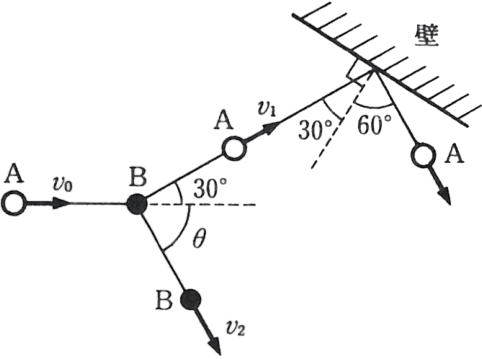
\includegraphics[width=12zw]{../graphs/se_1H_106.png}
\end{wrapfigure}
なめらかな水平面上に静止している小球Bに,質量$m$の小球Aが速さ$v_0$で衝突した.
衝突後の図のように,小球Aは進行方向に対し$30^\circ$の方向に進み,
小球Bは小球Aの衝突前の進行方向とゼロでない角$\theta$をなす方向に進んだ.
小球Aはその後水平面に垂直ななめらかな壁と,図のような角度で衝突してはね返った.
次の問いに答えよ.
\par}

\begin{enumerate}[(1)]
  \setlength{\leftskip}{-1.5zw}
  \setlength{\itemindent}{1zw}\setlength{\labelsep}{0.5zw}
  \setlength{\labelwidth}{1zw}\setlength{\leftmargin}{1zw}
  \item 小球AとBの衝突後の速さをそれぞれ$v_1,\,v_2$,またBの質量を$M$として,衝突における運動量保存則を,小球Aの衝突前の進行方向とそれに垂直な方向,それぞれの方向の成分について書け.
\end{enumerate}

衝突が弾性衝突であり,$v_1 = \dfrac{\sqrt{3}}{2}v_0$であることがわかったとする.
\begin{enumerate}[(1)]
  \setlength{\leftskip}{-1.5zw}
  \setlength{\itemindent}{1zw}\setlength{\labelsep}{0.5zw}
  \setlength{\labelwidth}{1zw}\setlength{\leftmargin}{1zw}
  \setcounter{enumi}{1}
  \item $v_0$と$m$を既知の量として,$v_0\,M,\,\theta$を求めよ.
  \item 衝突のとき小球AがBから受けた力積の大きさを求めよ.
  \item 衝突後,小球Bの得るエネルギーは,衝突前の小球Aの運動エネルギーの何倍か.
  \item 小球Aと壁との跳ね返り係数を求めよ.
  \item 小球Aが壁から受けた力積の大きさを求めよ.
  \item 小球Aが壁との衝突で失ったエネルギーを求めよ.
\end{enumerate}


% メモ
\begin{comment}

\end{comment}


%%%%%%%%%%%%%%%%%%
